\documentclass[12pt, letterpaper]{article}
\usepackage[utf8]{inputenc}
\usepackage{graphicx}  % Required for inserting images
\usepackage{amssymb}
\usepackage{amsmath}
\usepackage{enumitem}
\usepackage{fancyhdr}
\usepackage{geometry}

\graphicspath{ {./images/} }
\geometry{margin = 1in}
\renewcommand{\arraystretch}{1.5}
\linespread{2}

% Macros
\newcommand{\onespace}{\hspace*{1ex}}
\newcommand{\skipline}{\\[2\baselineskip]}
\newcommand{\tab}{\hspace*{4ex}}

\title{ECS 132 Term Project}
\author{\\ Ethan Wang, Briana Fedkiw, Priyal Patel}
\date{}
\pagestyle{fancy}
\setlength{\headheight}{41.68335pt}
\setlength\parindent{14pt}

\begin{document}

\maketitle

% Normal Family
\newpage
\noindent
\section*{Normal Distribution}
\normalsize
The chosen dataset of ``lawschoolbrief\$LSAT'' from the WAMfair section in the FairMLCourse repo recommended for use appears to represent a normal distribution PDF's shape \\
Initial Density Estimates\\
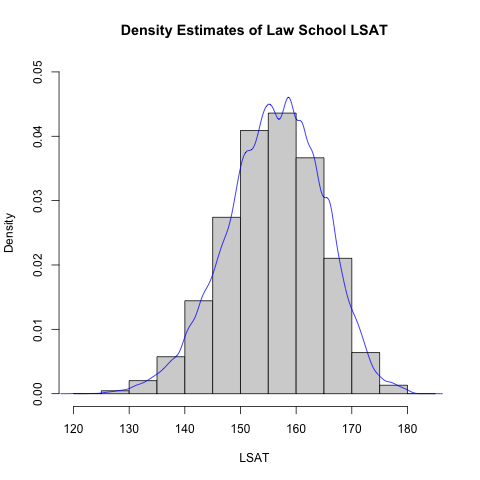
\includegraphics[scale=0.85]{Lawschool_LSAT_Density}\\
As seen above, there are some peculiarities. One is the how the histogram appears slightly skewed left, contradicting the fact that a normal distribution has zero skew. However, once the density function is superimposed, it has a similar shape to the bell curve of a normal distribution. \\
Another potential issue is how the density function is not fully smooth, with there being a dip before the peak. This dip most likely comes from sample variability. There might be some bias in different samples due to LSAT scores being based on people's performance. Since the dip is small, the trend generally still looks normal. To try to avoid the dip, one can play with the bandwidth of the density function. \\
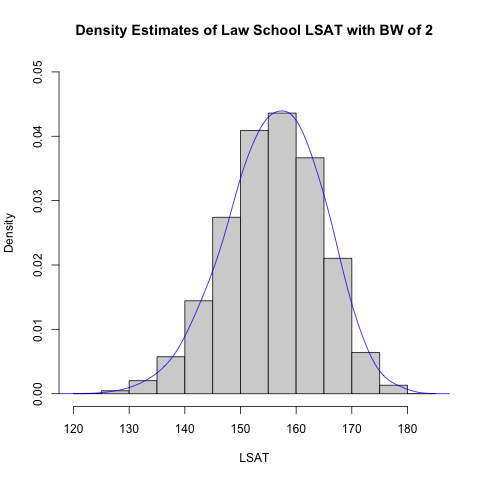
\includegraphics[scale=0.85]{Lawschool_LSAT_Density_bw}\\
A bandwidth of 2, caused the density function to mostly smooth out. However, finding the perfect bandwidth is subjective. So when using the estimating methods, it is best to compare their plots to both density graphs.
\newpage
\noindent
Using method of moments to estimate $\mu$ and $\sigma$
\begin{flalign*}
    E(X) &= \mu\\ 
    \overline{A} &= \mu\\
    \mu &= \frac{1}{n}\sum^{n}_{i=1}X_i \\
    &\approx 156.1726  \\
    Var(X) &= \sigma^2\\
    S^2 &= \sigma^2\\
    \sigma &= \sqrt(\frac{1}{n}\sum^{n}_{i=1}((X_i-\overline{A})^2)\\
    &\approx 8.622145 
\end{flalign*}
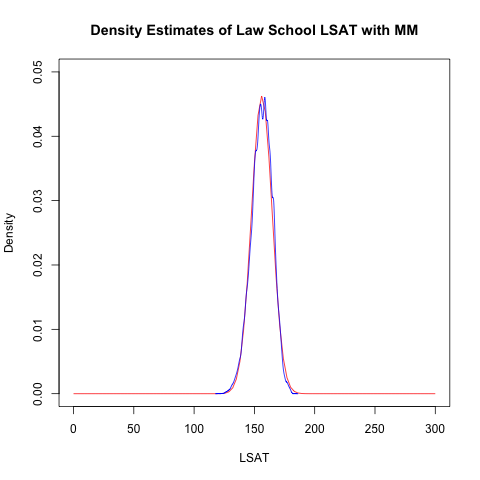
\includegraphics[scale=0.85]{Lawschool_LSAT_Density_mm} \\
\footnotesize
\**The blue curve is the plot of density(), the red curve uses the MM estimated $\mu$ and $\sigma$ in a plot of dnorm() \\
\normalsize
By using the sample mean $\overline{A}$ as an unbiased estimator of $\mu$ and $S^2$ as a biased estimator of $\sigma^2$, one can find $\mu$ and $\sigma$ from method of moments and graph the corresponding density function. As seen above, the graph using the estimated $\mu$ and $\sigma$ values closely matches the original density function of the data, implying that a normal distribution can approximate the population density of the data. However, one potential issue is the MM estimated curve peaks slightly before the density curve due to the dip. This can be addressed by changing bandwidth. Overall, the normal distribution is still fairly accurate at approximating the population density of the dataset. Now, change the bandwidth to 2.   \\
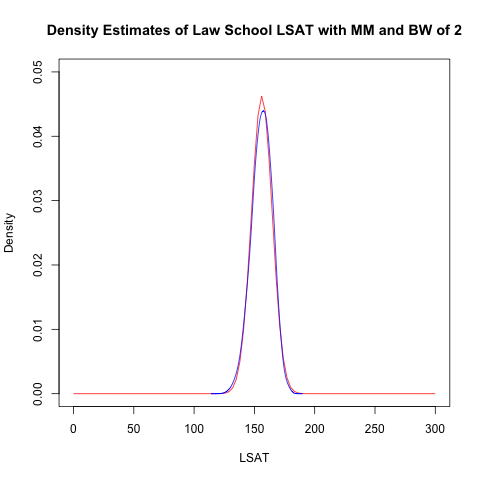
\includegraphics[scale=0.85]{Lawschool_LSAT_Density_mmbw} \\
Although the density graph is now smoother and the peaks are more aligned, its peak is now farther away from the peak of the MM estimated density graph. So, the MM estimated density graph with the default bandwidth is the better option. Due to how close the estimated density curve matches the dataset's density curve, a normal distribution is still a good approximator for the population density. 

\newpage
\noindent
Using method of maximum likelihood to estimate $\mu$ and $\sigma$\\
Log Likelihood Expression Derivation
\begin{flalign*}
    f_w(t) = \frac{1}{\sqrt(2pi)*\sigma}e^{-\frac{1}{2}(\frac{t-\mu}{\sigma})^2}
    \\[1\baselineskip]
    \prod^{n}_{i = 1} \frac{1}{\sqrt(2\pi)*\sigma}e^{-\frac{1}{2}(\frac{X_i-\mu}{\sigma})^2} &= \prod^{n}_{i = 1} \frac{1}{\sqrt(2\pi)*\sigma}e^{\frac{(X_i-\mu)^2}{-2\sigma^2}} = \prod^{n}_{i = 1} 2\pi^{-\frac{1}{2}}\sigma^{-1}e^{\frac{(X_i-\mu)^2}{-2\sigma^2}}
    \\[1\baselineskip]
    &= n\log(2\pi^{-\frac{1}{2}}) + n\log(\sigma^{-1}) + \sum^{n}_{i=1}(\frac{(X_i-\mu)^2}{-2\sigma^2})\\
    &= -\frac{n}{2}\log(2\pi) - n\log(\sigma) - \sum^{n}_{i=1}(\frac{(X_i-\mu)^2}{-2\sigma^2})
    \\[1\baselineskip]
    \text{MLE estimated } \mu &\approx 156.1725\ and\ \sigma \approx 8.621923
\end{flalign*}
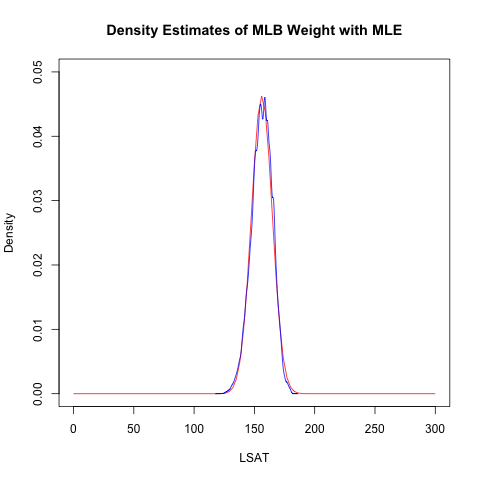
\includegraphics[scale=0.85]{Lawschool_LSAT_Density_mle}
\footnotesize
\\ \**The blue curve is the plot of density(), the red curve uses the MLE estimated $\mu$ and $\sigma$ in a plot of dnorm()
\normalsize
Both $\mu$ and $\sigma$ can be estimated from method of maximum likelihood and graphed accordingly. As seen above, the graph using the estimated $\mu$ and $\sigma$ values closely matches the original density function of the data, very similarly to the MM estimation. One can conclude that a normal distribution can approximate the population density of the data. Once again, the same issue of the location of the peak as seen in MM estimation exists in MLE. Now, change the bandwidth to 2 just like in MM.   \\
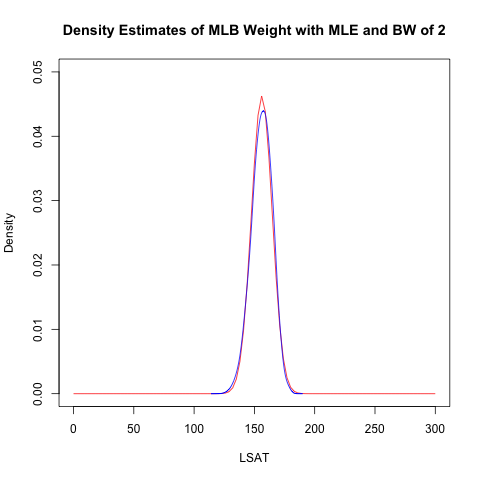
\includegraphics[scale=0.85]{Lawschool_LSAT_Density_mlebw} \\
Once again each case has its pros and cons, so it is hard to define which one is better to compare to MLE. However, the MLE estimated density curve with default bandwith appears to fit better. So, a normal distribution is still a good approximator for the population density when. 

\newpage
\noindent
In both the MM and MLE estimation methods, the values for $\mu$ and $\sigma$ were fairly close to one another. When looking at a normal distribution, one looks at the parameters of population mean and variance, $\mu$ and $\sigma^2$. From the data, the mean is $156.1726$ and the variance is $ 8.62219^2 \approx 74.34216$. Both our MM and MLE estimation methods had values of $\mu$ and $\sigma^2$ extremely close or even the same as the dataset. When looking at how much the estimated values differed from the dataset values, the difference was very small. For MM, the difference for $\mu$ was $\approx 0$ and for $\sigma$ was $\approx 0.000045$. For MLE, the difference for $\mu$ was $\approx 0.0001$ and for $\sigma$ was $\approx 0.000267$. Since the differences are so small, they support the fact that this dataset follows a normal distribution. \\
In summary, a normal distribution is a great approximator of population density for this dataset.  

% Exponential Family
\newpage
\noindent
\section*{Exponential Distribution}
\normalsize
The dataset ``adult\$capital\_gain" from fairml in the FairMLCourse repo seems to follow an exponential distribution PDF's shape \\
Initial Density Estimates\\
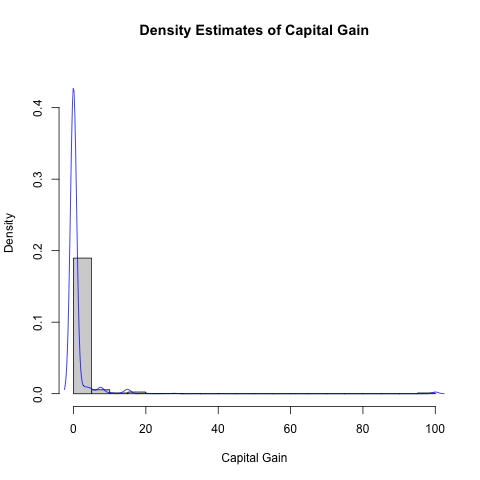
\includegraphics[scale=0.9]{capital_gain_density_estimates}
\newpage
\noindent
Using method of moments to estimate $\lambda$
\begin{flalign*}
    E(X) &= \frac{1}{\lambda}, L = \lambda\\
    \overline{A} &= \frac{1}{L}\\
    L &= \frac{\ 1\ }{\overline{A}}\\
    &\approx 0.916
\end{flalign*}
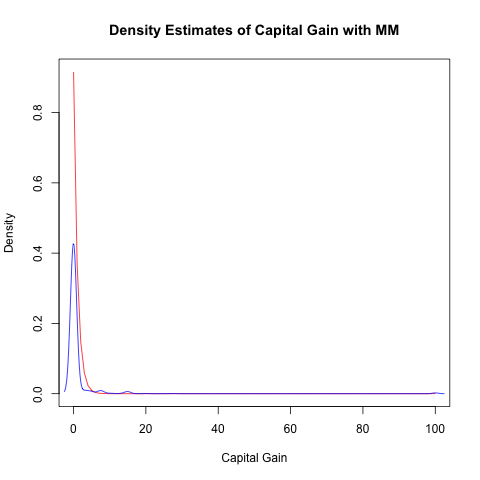
\includegraphics[scale=0.9]{capital_gain_mm}
\footnotesize
\\ \**The blue curve is the plot of density(), the red curve uses the MM estimated $\lambda$ in a plot of dexp()
\newpage
\noindent
\normalsize
Using method of maximum likelihood to estimate $\lambda$\\
Log Likelihood Expression Derivation
\begin{flalign*}
    \prod^{n}_{i = 1} {\lambda}e^{-{\lambda}X_i} &= {\lambda}^ne^{-{\lambda}\sum^{n}_{i=1}X_i}
    \\[1\baselineskip]
    \ln(\frac{\lambda^n}{e^{{\lambda}\sum^{n}_{i=1}X_i}}) &= \ln(\lambda^n) - \ln(e^{{\lambda}\sum^{n}_{i=1}X_i})\\
    &= n\ln(\lambda) - {\lambda}\sum^{n}_{i=1}X_i
    \\[1\baselineskip]
    \text{MLE estimated } \lambda &\approx 0.916
\end{flalign*}
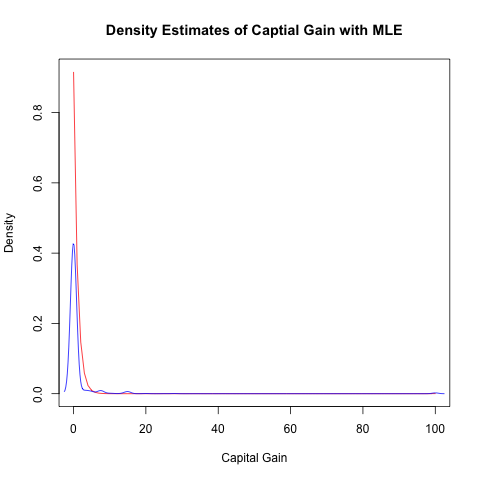
\includegraphics[scale=0.9]{capital_gain_mle}
\footnotesize
\\ \**The blue curve is the plot of density(), the red curve uses the MLE estimated $\lambda$ in a plot of dexp()
\newpage
\noindent
\normalsize
In Professor Matloff's fastStat lesson, ``MLEMM: General Methods of Estimation," both the method of 
moments estimator and the maximum likelihood estimator for the parameter $\lambda$ of an exponential 
distribution was $\frac{\ 1\ }{\overline{A}}$. However, the mle function from the stats4 
library was used to estimate $\lambda$ instead of using $\frac{\ 1\ }{\overline{A}}$ directly for the 
maximum likelihood estimator, both for consistency across our work and as an extra verification measure. 
As expected, both estimators yielded a result of about 0.916. The graph of the exponential distribution 
PDF using the estimated $\lambda$ closely follows that of the density curve of the data, which suggests 
that an exponential distribution is a suitable approximation for the population density of this dataset. 
An initial concern was the fact that there was a peak in the original density graph rather than a pure 
exponential curve and that there was a positive, nonzero density region to the left of zero. However, the 
exponential distribution is still believed to approximate the dataset well since there are no actual 
capital gain values less than zero in the dataset and a Google search revealed that the density region to 
the left of zero in the graph is a result of the kernel density estimation the density function does for 
the capital gain values equal to zero.


% Gamma Family
\newpage
\noindent
\section*{Gamma Distribution}
\normalsize
The dataset ``prgeng\$age" from qeML in the FairMLCourse repo seems to follow a gamma distribution PDF's shape \\
Initial Density Estimates\\
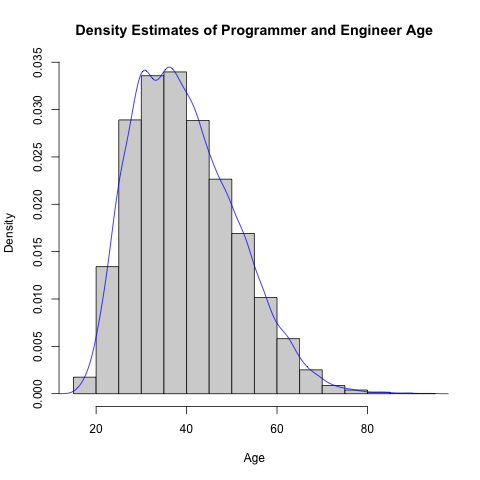
\includegraphics[scale=0.9]{prgeng_age_density_estimates}
\newpage
\noindent
Using method of moments to estimate $\lambda$ and $r$
\begin{flalign*}
    E(X) &= \frac{r}{\lambda}, L = \lambda, R = r\\
    \sigma^2 &= \frac{r}{\lambda^2}\\
    \overline{A} &= \frac{R}{L}\\
    S^2 &= \frac{R}{L^2}\\
    \\[1\baselineskip]
    R &= L\overline{A}\\
    S^2 &= \frac{L\overline{A}}{L^2}\\
    &= \frac{\overline{A}}{L}\\
    L &= \frac{\overline{A}}{S^2}\\
    &\approx 0.314\\
    R &\approx 12.421
\end{flalign*}
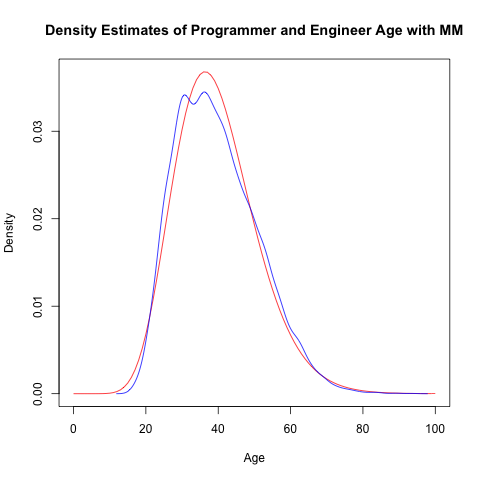
\includegraphics[scale=0.9]{prgeng_age_mm}
\footnotesize
\\ \**The blue curve is the plot of density(), the red curve uses the MM estimated {$\lambda$} and $r$ in a plot of dgamma()
\newpage
\noindent
\normalsize
Using method of maximum likelihood to estimate $\lambda$ and r\\
Log Likelihood Expression Derivation
\begin{flalign*}
    \prod^{n}_{i = 1} \frac{{\lambda}^rX_i^{r-1}}{\Gamma(r)e^{{\lambda}X_i}} &= (\frac{\lambda^r}{\Gamma(r)})^n \ast \prod^n_{i=1}X_i^{r-1} \ast \frac{1}{e^{{\lambda}\sum^n_{i=1}X_i}}
    \\[1\baselineskip]
    \ln((\frac{\lambda^r}{\Gamma(r)})^n \ast \prod^n_{i=1}X_i^{r-1} \ast \frac{1}{e^{{\lambda}\sum^n_{i=1}X_i}}) &= \ln(\lambda^{rn}) + \ln(\prod^n_{i=1}X_i^{r-1}) - \ln(e^{{\lambda}\sum^{n}_{i=1}X_i}) - \ln((\Gamma(r))^n)\\
    &= rn\ln(\lambda) + (r-1)\sum^n_{i=1}\ln(X_i) - {\lambda}\sum^{n}_{i=1}X_i - n\ln(\Gamma(r))
    \\[1\baselineskip]
    \text{MLE estimated } \lambda &\approx 0.320\\
    \text{MLE estimated } r &\approx 12.643
\end{flalign*}
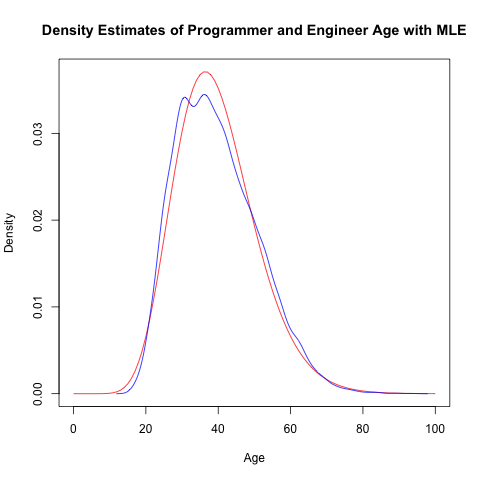
\includegraphics[scale=0.9]{prgeng_age_mle}
\footnotesize
\\ \**The blue curve is the plot of density(), the red curve uses the MLE estimated {$\lambda$} and $r$ in a plot of dgamma()
\newpage
\noindent
\normalsize
For the dataset chosen to be approximated by a gamma distribution, the estimated values for $\lambda$ and $r$ 
have little difference from one method of forming estimators to the other. The graphs of the gamma 
distribution PDF using the estimated $\lambda$ and $r$ parameters for each estimation fit the density 
curve of the dataset well, suggesting that a gamma distribution is a suitable approximation for the 
population density of this dataset. One concern is that the peaks of both PDFs are slightly to the right 
of the one in the original density graph. Since the difference in peak locations is pretty small, the 
suitability of the gamma distribution in approximating the population density of the dataset remains 
unchanged.
\\[0.5\baselineskip]
Another concern was the slight dip in the peak of the density graph of the dataset. While playing with the 
bandwidth parameter, a bandwidth value of four got rid of the dip, as depicted below.
\\
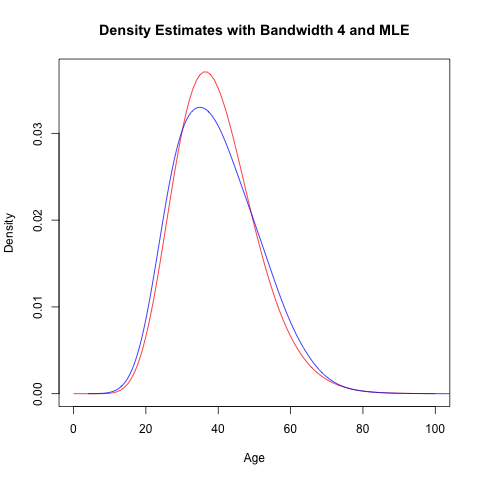
\includegraphics[scale=0.9]{prgeng_age_bandwidth_4}
\footnotesize
\\ \**The blue curve is the plot of density() with bw=4, the red curve is the same MLE graph as above \\
\normalsize
However, a bandwidth of four felt like too much smoothing since it is very likely that this small dip is a 
result of sample variability. The reasoning behind this is one, the dip is small enough so that it does 
not create two peaks, and two, this dataset involves the ages of programmers and engineers, and it seems 
unlikely that there would be a sudden downward trend in the number of programmers and engineers around the 
age of 35. This bandwidth setting also makes the MLE and MM graphs less fitting.

%Beta
\newpage
\noindent
\section*{Beta Distribution}
\normalsize
The dataset referenced was "austinweather.csv" from Gruben M on kaggle from $https://www.kaggle.com/datasets/grubenm/austin-weather$.\\ To select a data set, the first criteria checked was the data was contained within [0,1], a primary characteristic of a beta distribution. From the data sets that met the first criteria, the sample with the largest size was selected, n=1317. The Low Humidity Percentage was used for the analysis. Selection bias was present due to two days not having data, which were directly excluded from the data set utilized.\\
Initial Density Estimates\\
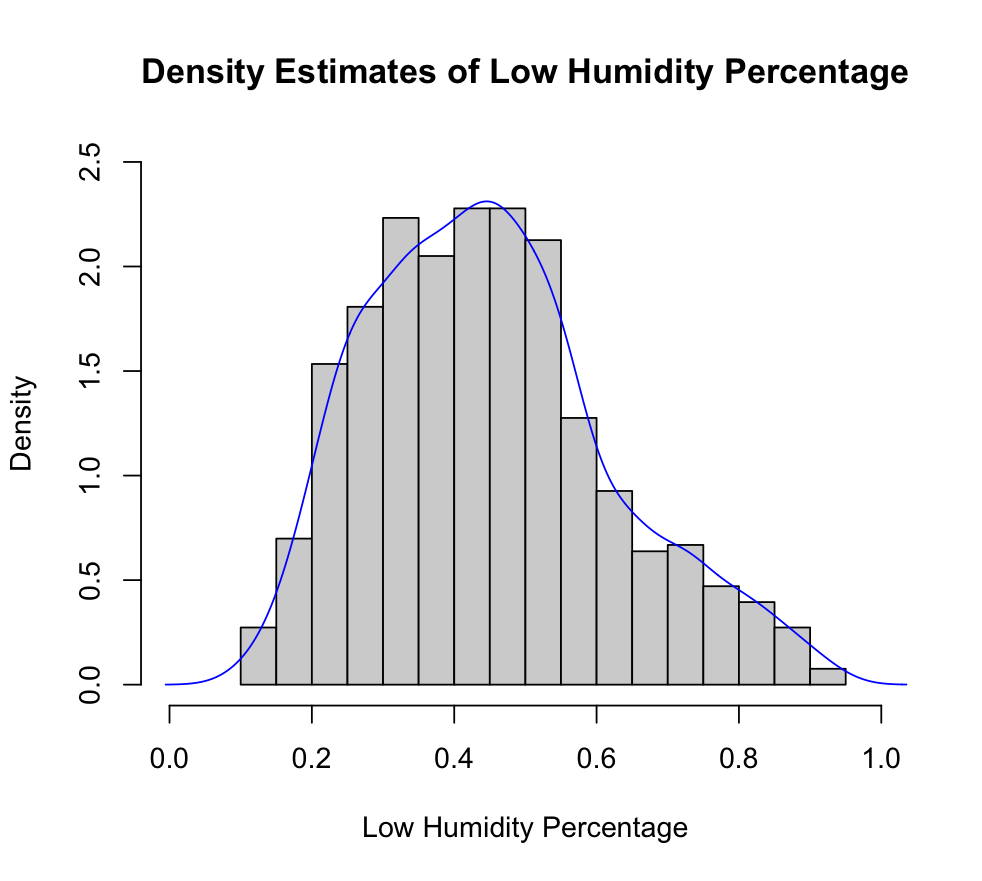
\includegraphics[scale=0.41]{austinweather_densityestimates.png}
\footnotesize
\\ \**The blue curve is the plot of density() \\
\vstretch{1.2}{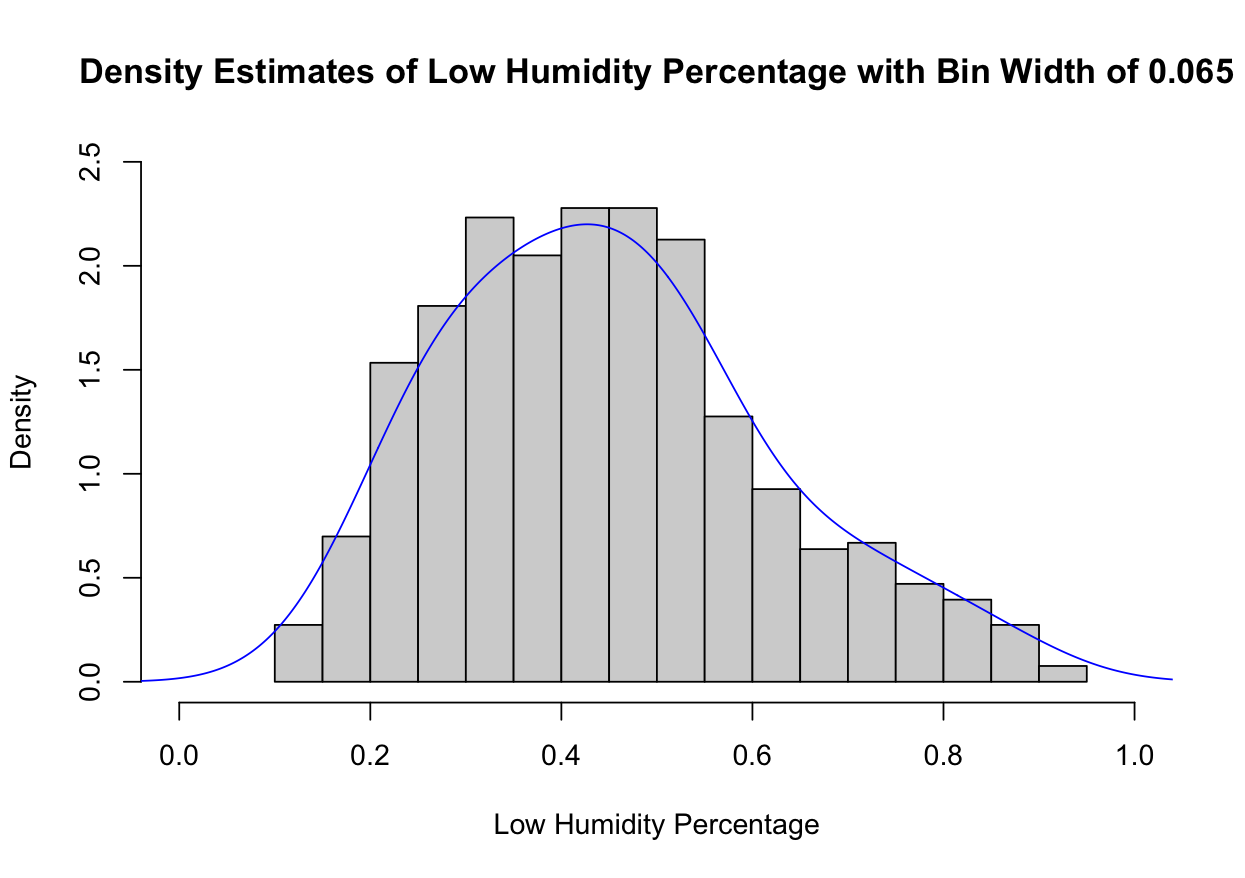
\includegraphics[scale=0.32]{austinweather_densitybw0.065.png}}
\footnotesize
\\ \**The blue curve is the plot of density() with bw=0.065\\
As seen above, the histogram appears slightly skewed to the left and density curve is not fully smooth. The small dips in the curve are due to sample variability and by changing the bandwidth to 0.065 this provides a better fit with the MM and MLE graphs.\\
Using method of moments to estimate ${\alpha}$ and ${\beta}$:\\
$E(X) = mean(austinweather\$HumidityLowPercent) = 0.44958998$\\
$var(X) = var(austinweather\$HumidityLowPercent) = 0.02881381$\\
To find the long run average, $E(X) = {\alpha / (\alpha + \beta)}$.\\ 
To find variance, $var(X) = {(\alpha*\beta)/ ((\alpha + \beta)^2*(\alpha + \beta + 1)}$.\\
To solve for $\alpha$ and $\beta$, you can rewrite the expected value equation as $\beta = (\alpha/E(X)) - \alpha$. \\
Then, replace $\beta$ written in terms of $\alpha$ into the variance equation as \\ $var(X) = {(\alpha*((\alpha/E(X)) - \alpha))/ ((\alpha + ((\alpha/E(X)) - \alpha))^2*(\alpha + ((\alpha/E(X)) - \alpha) + 1)}$.\\ ${\text{MM estimated } \alpha \approx} 3.41157 \tab {\text{MM estimated } \beta \approx} 4.176611$\\
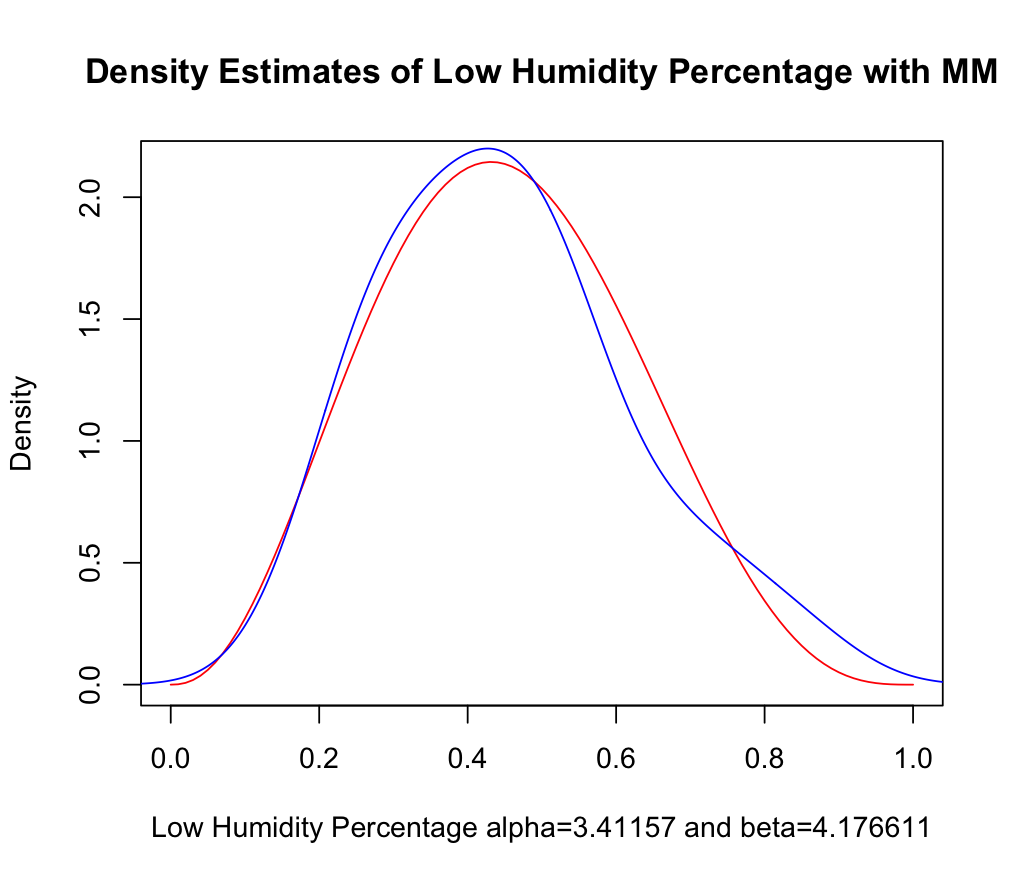
\includegraphics[scale=0.37]{austinweather_mm.png}
\footnotesize
\\ \**The blue curve is the plot of density() with bw=0.065, the red curve uses the MM estimated ${\alpha}$ and ${\beta}$ in a plot of dbeta() \\
Using method of maximum likelihood to estimate ${\alpha}$ and ${\beta}$:\\
Log Likelihood Expression Derivation
\begin{flalign*}
    \prod^{n}_{i = 1} \frac{{\Gamma(\alpha + \beta)}}{\Gamma(\alpha)\Gamma(\beta)}{X_i^{\alpha-1}(1-X_i)^{\beta-1}} &= (\frac{{\Gamma(\alpha + \beta)}}{\Gamma(\alpha)\Gamma(\beta)})^n \ast \prod^n_{i=1}X_i^{\alpha-1} \ast \prod^n_{i=1}(1-X_i)^{\beta-1}
    \\ &= \ln((\frac{{\Gamma(\alpha + \beta)}}{\Gamma(\alpha)\Gamma(\beta)})^n \ast \prod^n_{i=1}X_i^{\alpha-1} \ast \prod^n_{i=1}(1-X_i)^{\beta-1}) \\ &= \ln((\frac{{\Gamma(\alpha + \beta)}}{\Gamma(\alpha)\Gamma(\beta)})^n) + \ln(\prod^n_{i=1}X_i^{\alpha-1}) + \ln(\prod^n_{i=1}(1-X_i)^{\beta-1})
    \\ &= \ln({\Gamma(\alpha + \beta)}^n) - \ln(({\Gamma(\alpha)\Gamma(\beta)})^n) + \ln(\prod^n_{i=1}X_i^{\alpha-1}) + \ln(\prod^n_{i=1}(1-X_i)^{\beta-1}) \\ &= n\ln({\Gamma(\alpha + \beta)}) - n\ln({\Gamma(\alpha)}) - n\ln({\Gamma(\beta)}) + ({\alpha-1})\sum^{n}_{i=1}\ln(X_i) + ({\beta-1})\sum^{n}_{i=1}\ln(1-X_i)\\
    \text{MLE estimated } \alpha &\approx 3.447276 \\ 
    \text{MLE estimated } \beta &\approx 4.150187
\end{flalign*}
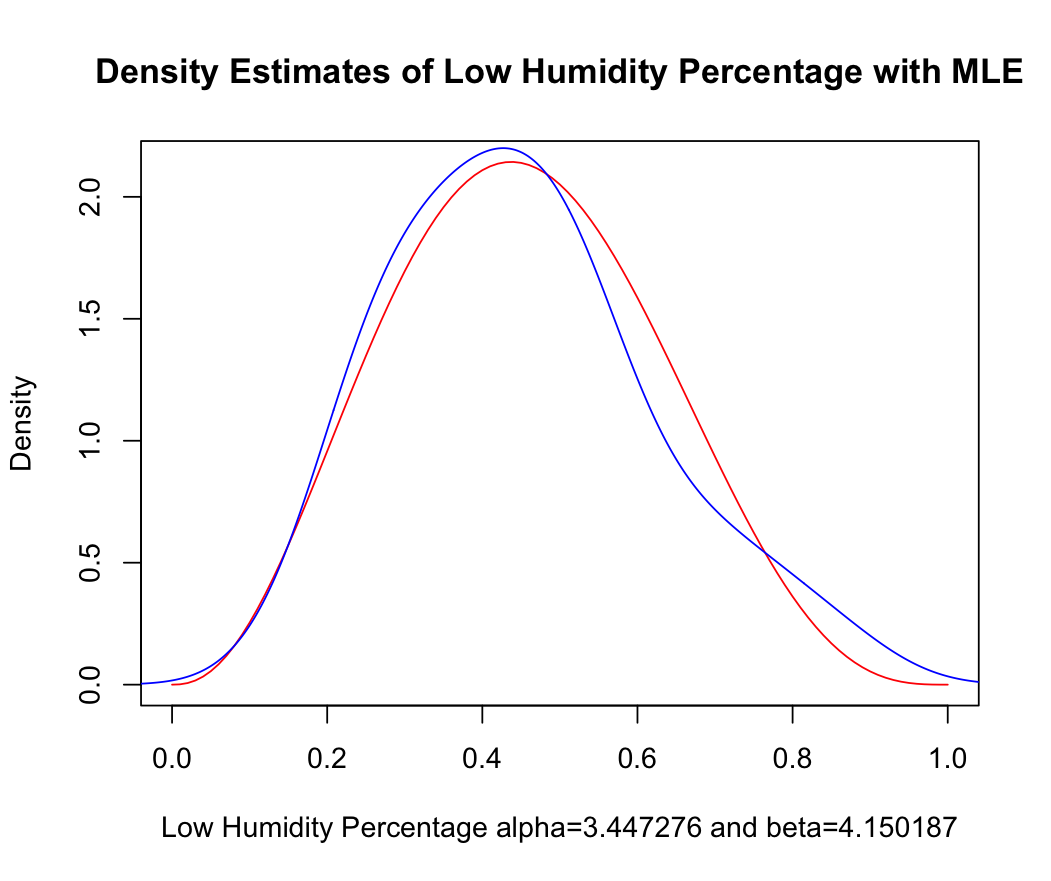
\includegraphics[scale=0.34]{austinweather_mle.png}
\footnotesize
\\ \**The blue curve is the plot of density() with bw=0.065, the red curve uses the MLE estimated ${\alpha}$ and ${\beta}$ in a plot of dbeta() \\
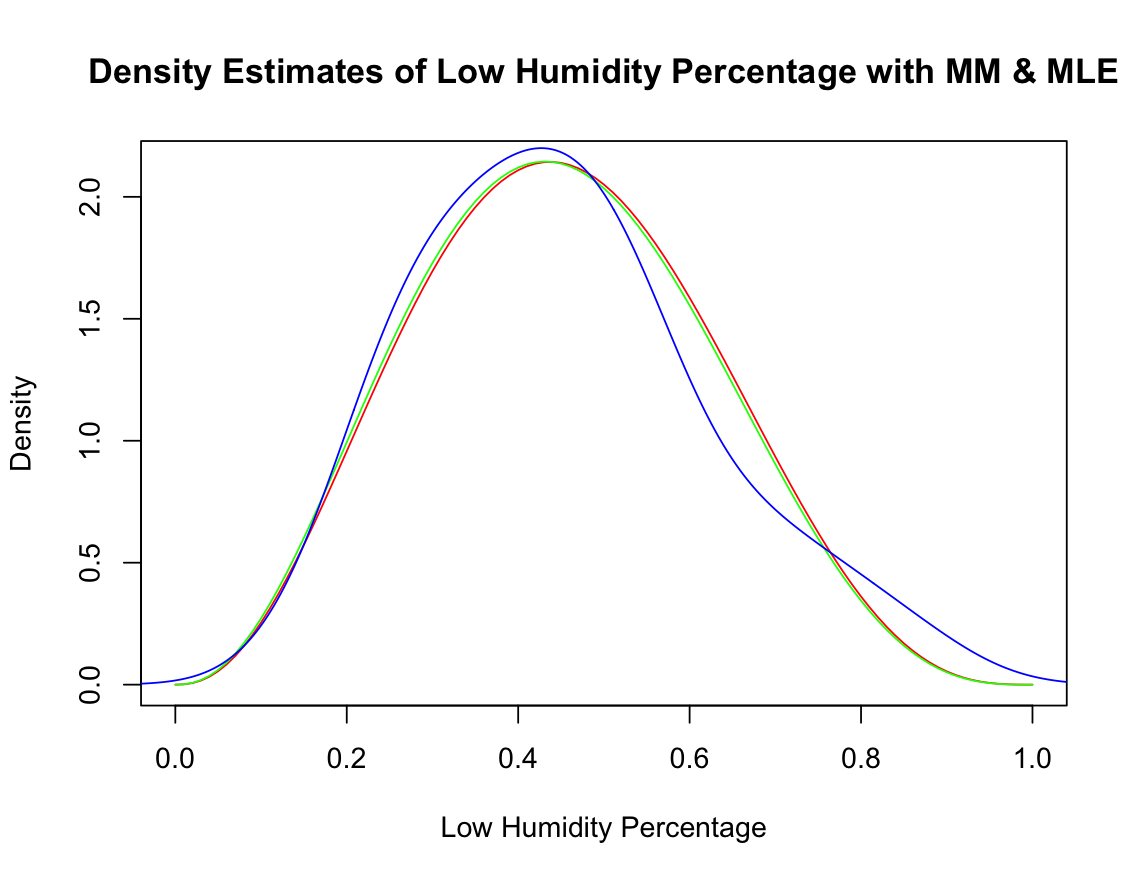
\includegraphics[scale=0.32]{austinweather_mmmle.png}
\footnotesize
\\ \**The blue curve is the plot of density() with bw=0.065, the red curve uses the MLE estimated ${\alpha}$ and ${\beta}$ in a plot of dbeta(), the green curves uses the MM estimated ${\alpha}$ and ${\beta}$ in a plot of dbeta() \\
\normalsize After superimposing the both MM and MLE estimation beta density curves on the density estimation, the curves all appeared to be concave down and the input x-values were contained within [0,1]. Both density estimate with MM and MLE graphs provide evidence that the density curve for the data set approximately represents a beta distribution. However, it is important to note that the MM and MLE estimation beta density curves both lean towards symmetric more than the density curve. There are smaller densities for higher percentage of low humidity for the density curve, exemplifying the variability of low humidity in Austin. For the smaller percentage of low humidity for the density curve, the density estimate with MM and MLE curves closer approximate the density curve for the data set. There is a small difference for the estimated values for ${\alpha}$ and ${\beta}$ between the MM and MLE estimation methods. For MM method estimates, ${\alpha \approx} 3.41157$ and ${\beta \approx} 4.176611$. For MLE method estimates, ${\alpha \approx} 3.447276$ and ${\beta \approx} 4.150187$. The graph that contains all the density curves demonstrates the close estimates of ${\alpha}$ and ${\beta}$ by both MM and MLE methods, proving that both are similar comparisons to determine if the density curve of the data set approximates a beta distribution. Further, the number of successes is described as ${\alpha -1}$ and the number of failures as ${\beta - 1}$. The estimated ${\alpha}$ and ${\beta}$ from the MM and MLE methods reveal the approximate number of successes and failures. Based on ${\alpha}$ and ${\beta}$ values, a beta distribution can take a diverse array of shapes. The concave down and approximately bell-shaped look of all the curves demonstrates that the density curve for the data set compared to the beta density curves from estimation methods MM and MLE parameters approximately fits a beta distribution.\\ 

% Contribution Section
\newpage
\begin{center}
    \section*{Team Member Contributions}
\end{center}

\normalsize
Briana Fedkiw
\begin{itemize}[leftmargin=50pt]
  \item Normal distribution (data and analysis)
  \item R code in normal.R
\end{itemize}

Ethan Wang
\begin{itemize}[leftmargin=50pt]
  \item Exponential and gamma distributions (data and analysis)
  \item R code in exp\_and\_gamma.R
\end{itemize}

Priyal Patel
\begin{itemize}[leftmargin=50pt]
  \item Beta distribution (data and analysis)
  \item R code in beta.R
\end{itemize}

Group
\begin{itemize}[leftmargin=50pt]
  \item Presented our datasets to each other and explained why the distributions were a good fit for the datasets
  \item Worked together on the derivations of the method of moments estimators and maximum likelihood estimators for our distributions
\end{itemize}

\end{document}

\end{document}

